\documentclass[]{article}
\usepackage{lmodern}
\usepackage{amssymb,amsmath}
\usepackage{ifxetex,ifluatex}
\usepackage{fixltx2e} % provides \textsubscript
\ifnum 0\ifxetex 1\fi\ifluatex 1\fi=0 % if pdftex
  \usepackage[T1]{fontenc}
  \usepackage[utf8]{inputenc}
\else % if luatex or xelatex
  \ifxetex
    \usepackage{mathspec}
  \else
    \usepackage{fontspec}
  \fi
  \defaultfontfeatures{Ligatures=TeX,Scale=MatchLowercase}
\fi
% use upquote if available, for straight quotes in verbatim environments
\IfFileExists{upquote.sty}{\usepackage{upquote}}{}
% use microtype if available
\IfFileExists{microtype.sty}{%
\usepackage[]{microtype}
\UseMicrotypeSet[protrusion]{basicmath} % disable protrusion for tt fonts
}{}
\PassOptionsToPackage{hyphens}{url} % url is loaded by hyperref
\usepackage[unicode=true]{hyperref}
\hypersetup{
            pdftitle={Satellite field verification results},
            pdfauthor={Keith Bouma-Gregson \textbar{} CA State Waterboards},
            pdfborder={0 0 0},
            breaklinks=true}
\urlstyle{same}  % don't use monospace font for urls
\usepackage[margin=1in]{geometry}
\usepackage{longtable,booktabs}
% Fix footnotes in tables (requires footnote package)
\IfFileExists{footnote.sty}{\usepackage{footnote}\makesavenoteenv{long table}}{}
\usepackage{graphicx,grffile}
\makeatletter
\def\maxwidth{\ifdim\Gin@nat@width>\linewidth\linewidth\else\Gin@nat@width\fi}
\def\maxheight{\ifdim\Gin@nat@height>\textheight\textheight\else\Gin@nat@height\fi}
\makeatother
% Scale images if necessary, so that they will not overflow the page
% margins by default, and it is still possible to overwrite the defaults
% using explicit options in \includegraphics[width, height, ...]{}
\setkeys{Gin}{width=\maxwidth,height=\maxheight,keepaspectratio}
\IfFileExists{parskip.sty}{%
\usepackage{parskip}
}{% else
\setlength{\parindent}{0pt}
\setlength{\parskip}{6pt plus 2pt minus 1pt}
}
\setlength{\emergencystretch}{3em}  % prevent overfull lines
\providecommand{\tightlist}{%
  \setlength{\itemsep}{0pt}\setlength{\parskip}{0pt}}
\setcounter{secnumdepth}{0}
% Redefines (sub)paragraphs to behave more like sections
\ifx\paragraph\undefined\else
\let\oldparagraph\paragraph
\renewcommand{\paragraph}[1]{\oldparagraph{#1}\mbox{}}
\fi
\ifx\subparagraph\undefined\else
\let\oldsubparagraph\subparagraph
\renewcommand{\subparagraph}[1]{\oldsubparagraph{#1}\mbox{}}
\fi

% set default figure placement to htbp
\makeatletter
\def\fps@figure{htbp}
\makeatother

\usepackage{amsmath}

\title{Satellite field verification results}
\author{Keith Bouma-Gregson \textbar{} CA State Waterboards}
\date{January 2, 2020}

\begin{document}
\maketitle

\subsection{\texorpdfstring{\textbf{Introduction}}{Introduction}}\label{introduction}

The CA State Waterboards contracted with the San Francisco Estuary
Institute (SFEI) to use satellite imagery to estimate cyanobacterial
abundance. Algorithms to estimate cyanobacterial abundance in the
surface waters of Lake Erie have been developed by Wynne et al. (2008)
and Lunetta et al. (2015). Working with NOAA staff, SFEI applied these
algorithms to waterbodies in California.

To better understand the performance of the satellite tool, field
verification sampling was conducted in 2019. This document presents the
initial results from the 2019 field verification effort.

\subsection{\texorpdfstring{\textbf{Methods}}{Methods}}\label{methods}

\paragraph{\texorpdfstring{\emph{Field
sampling}}{Field sampling}}\label{field-sampling}

Seven sampling events occurred at four different waterbodies from August
1 to October 8, 2019 (Table 1). Only Clear Lake had satellite pixels
with positive CI\textsubscript{cyano} values on the sampling days. There
had been blooms at San Pablo Reservoir and Lake San Antonio, but they
had dissipated to non-detects on the satellite by the time we were able
to sample them. Lake Almanor was chosen due to its higher elevation and
previous questionable CI\textsubscript{cyano} values generated by MERIS
imagery.

\begin{longtable}[]{@{}lllll@{}}
\caption{\textbf{Table 1.} Waterbody information}\tabularnewline
\toprule
Name & County & Sampling date & Surface area (km\textsuperscript{2}) &
Elevation (m)\tabularnewline
\midrule
\endfirsthead
\toprule
Name & County & Sampling date & Surface area (km\textsuperscript{2}) &
Elevation (m)\tabularnewline
\midrule
\endhead
Clear Lake & Lake & Aug-7, Aug-16, Oct-8 & 180 & 432\tabularnewline
Lake Almanor & Plumas & Aug-15 & 113 & 1373\tabularnewline
Lake San Antonio & Monterrey & Aug-1 & 23 & 245\tabularnewline
San Pablo Reservoir & Contra Costa & Aug-12 & 60 & 96\tabularnewline
\bottomrule
\end{longtable}

Field sampling occurred on the same day as the Sentinel-3a flyover. In a
waterbody three pixels were selected for sampling. Within a pixel, three
samples were collected, for a total of nine measurement sites (Fig. 1).
At each sampling point, a Malvern Panalytical Fieldspec Handheld2 Pro
radiometer was used to collect radiance data, which can be converted to
a CI\textsubscript{cyano} equivalent value for comparison to the
satellite data. Each reading involved collecting ten measurements at 1
nm wavelength resolution from 300-900 nms, which were then averaged into
a single value per nm for the reading. Readings were taken on a
calibrated 10\% Spectralon reflectance plate, the water, and the sky.
All readings were taken 40-45 degrees altitude and 115-130 degrees
alzimuth from the sun. Triplicate plate, water, and sky readings were
collected at each sampling site. Additionally, Secchi depth was
measured, and depth integrated grab samples (1 m) for chlorophyll-a were
collected at each sampling site. Chlorophyll-a samples were immediately
chilled on ice in a cooler and filtered onto 0.7 micrometer (Whatman
GF/C) filters back on shore. The filters were then wrapped in aluminum
foil and frozen until fluorometric analysis.

\includegraphics[width=0.3\linewidth]{../Data/Figures_output/Map_Figure}

\textbf{Figure 1.} Sampling maps of Lake San Antonio. Left panel) Entire
lake showing the pixel locations for satellite imagery. Colors show the
locations of the sampling pixels. Right panel) Zoom in of the sampling
area showing the three different sampling sites within each of the three
pixels. Numbers are the pixel ID for the satellite.

\paragraph{\texorpdfstring{\emph{Field remote sensed reflectance
calculations}}{Field remote sensed reflectance calculations}}\label{field-remote-sensed-reflectance-calculations}

The raw radiance values (W/m\textsuperscript{2}/nm/sr) from the
radiometer were converted to remote sensed reflectance
(R\textsubscript{rs}) values per nm/sr using the program
\texttt{test\_asd\_group.exe} provided to the Waterboards by NOAA staff.
The calculations take the plate, water, and sky readings and calculate
R\textsubscript{rs} based on equation 4 in Mobley 1999: \[
\begin{equation}
R_{rs} = \frac{L_{water} - \rho * L_{sky}}{L_{plate}}
\end{equation}
\] \{\#eq:1\} Where L indicates the radiance values, and \(\rho\)
represents the proportion of sky radiance that is reflected by the
water's surface.

\paragraph{\texorpdfstring{\emph{Cyanobacterial index
calculations}}{Cyanobacterial index calculations}}\label{cyanobacterial-index-calculations}

The R\textsubscript{rs} values were used to calculate the cyanobacterial
indices CI and CI\textsubscript{cyano}. The CI value is derived from the
spectral shape (SS) at 681 nm and is calculated with equation 1 in Wynne
et al. 2008: \[
\begin{equation}
SS(681) = rrs681 - rrs665 - (rrs709 - rrs665) * \frac{681-665}{709-665}
\end{equation}
\] \{\#eq:2\} More negative SS(681) values represent higher
cyanobacterial abundances in the surface waters of a pixel. To transform
it into positive values the SS(681) is converted to CI by: \[
\begin{equation}
CI = -1*SS(681)
\end{equation}
\] \{\#eq:3\} CI values \textless{}0 indicate no cyanobacteria present.
However, certain water conditions can generate positive CI values, even
when there are no cyanobacteria present. To reduce the frequency of
false positives, an exclusionary criteria (Matthews et al. 2012 and
Lunetta et al 2015) based on the spectral shape at 665 nm is used: \[
\begin{equation}
SS(665) = rrs665 - rrs620 + (rrs620 - rrs681) * \frac{665-620}{681-620}
\end{equation}
\] \{\#eq:4\} When SS(665) is \textgreater{}0 it indicates cyanobacteria
present in the water and when it is \textless{}0, cyanobacteria is
predicted to be absent. SS(665) is then transformed into an exclusion
criteria value of 1 when SS(665) \textgreater{}0 and 0 when SS(665)
\textless{}0. \[
\begin{equation}
  f(SS(665))=\begin{cases}
    1, & \text{if SS(665) > 0}.\\  
    0, & \text{if SS(665) < 0}.
  \end{cases}
\end{equation}
\] \{\#eq:5\} The CI value and f(SS(665)) are combined to create a new
indice called CI\textsubscript{cyano} which is calculated by: \[
\begin{equation}
CI_{cyano} = f(SS(665)) * CI
\end{equation}
\] \{\#eq:6\}

This will render all measurements with f(SS(665)) = 0 as non-detects,
even if they had a positive CI value.

\paragraph{\texorpdfstring{\emph{Satellite data
calculations}}{Satellite data calculations}}\label{satellite-data-calculations}

The satellite CI\textsubscript{cyano} value is calculated from the OLCI
sensor on Sentinel-3a satellite. The value is calculated by NOAA using
top-of-atmosphere reflectance values applied to equations 1-5 above
(Wynne et al. 2018). NOAA delivers the CI\textsubscript{cyano} product
for each pixel as an integer ranging in values 0-250, corresponding to
increasing CI\textsubscript{cyano} value. The pixel integer value is
converted to CI\textsubscript{cyano} with: \[
\begin{equation}
CI_{cyano} = 10^{0.012 * PixInteger - 4.2}
\end{equation}
\] \{\#eq:7\}

CI\textsubscript{cyano} has a range of 0.000063 - 0.063270. To make
these values easier to work with, SFEI and the CA Waterboards then
multiply CI\textsubscript{cyano} by a constant to make the values easier
to work with by putting them on a scale of 1-1000. This index is called
CI\textsubscript{mod} and calculated by: \[
\begin{equation}
CI_{mod} = CI_{cyano} * 15805.18
\end{equation}
\] \{\#eq:8\}

\subsection{\texorpdfstring{\textbf{Results}}{Results}}\label{results}

\paragraph{\texorpdfstring{\emph{Lake
conditions}}{Lake conditions}}\label{lake-conditions}

Lakes ranged in phytoplankton concentrations, with median chl-a
concentrations ranging from 1-40 ug/L (Fig. 2) and Secchi depths ranged
from \textless{}1 - 4.5 meters (Fig. 3). Only in Clear Lake were
cyanobacterial colonies visible (Fig. 4), however, microscopic analysis
of samples did identify cyanobacterial taxa in some waterbodies,
including \emph{Dolichospermum}, \emph{Microcystis}, and
\emph{Gloeotrichia} (Table 2). No cell counts of cyanobacteria abundance
were performed.

\begin{figure}

{\centering \includegraphics[width=0.6\linewidth]{../Data/Figures_output/chla} 

}

\end{figure}

\textbf{Figure 2.} Chlorophyll-a concentrations at sampling locations in
waterbodies. (Note: data was not collected for Clear Lake on Aug-16 and
Oct-8).

\begin{figure}

{\centering \includegraphics[width=0.6\linewidth]{../Data/Figures_output/secchi} 

}

\end{figure}

\textbf{Figure 3.} Secchi depth at sampling locations in waterbodies.
(Note: data was not collected for Clear Lake on Aug-16 and Oct-8).

\begin{longtable}[]{@{}lll@{}}
\caption{\textbf{Table 2.} Microscopic cyanobacteria
identification.}\tabularnewline
\toprule
Name & Sampling\_date & Cyanobacteria\tabularnewline
\midrule
\endfirsthead
\toprule
Name & Sampling\_date & Cyanobacteria\tabularnewline
\midrule
\endhead
Clear Lake & Aug-7 & \emph{Microcystis}, \emph{Gloeotrichia},
\emph{Dolichospermum}\tabularnewline
Clear Lake & Aug-16 & No data\tabularnewline
Clear Lake & Oct-8 & No data\tabularnewline
Lake Almanor & Aug-15 & None\tabularnewline
Lake San Antonio & Aug-1 & \emph{Dolichospermum}\tabularnewline
San Pablo Reservoir & Aug-12 & \emph{Dolichospermum}\tabularnewline
\bottomrule
\end{longtable}

\begin{figure}
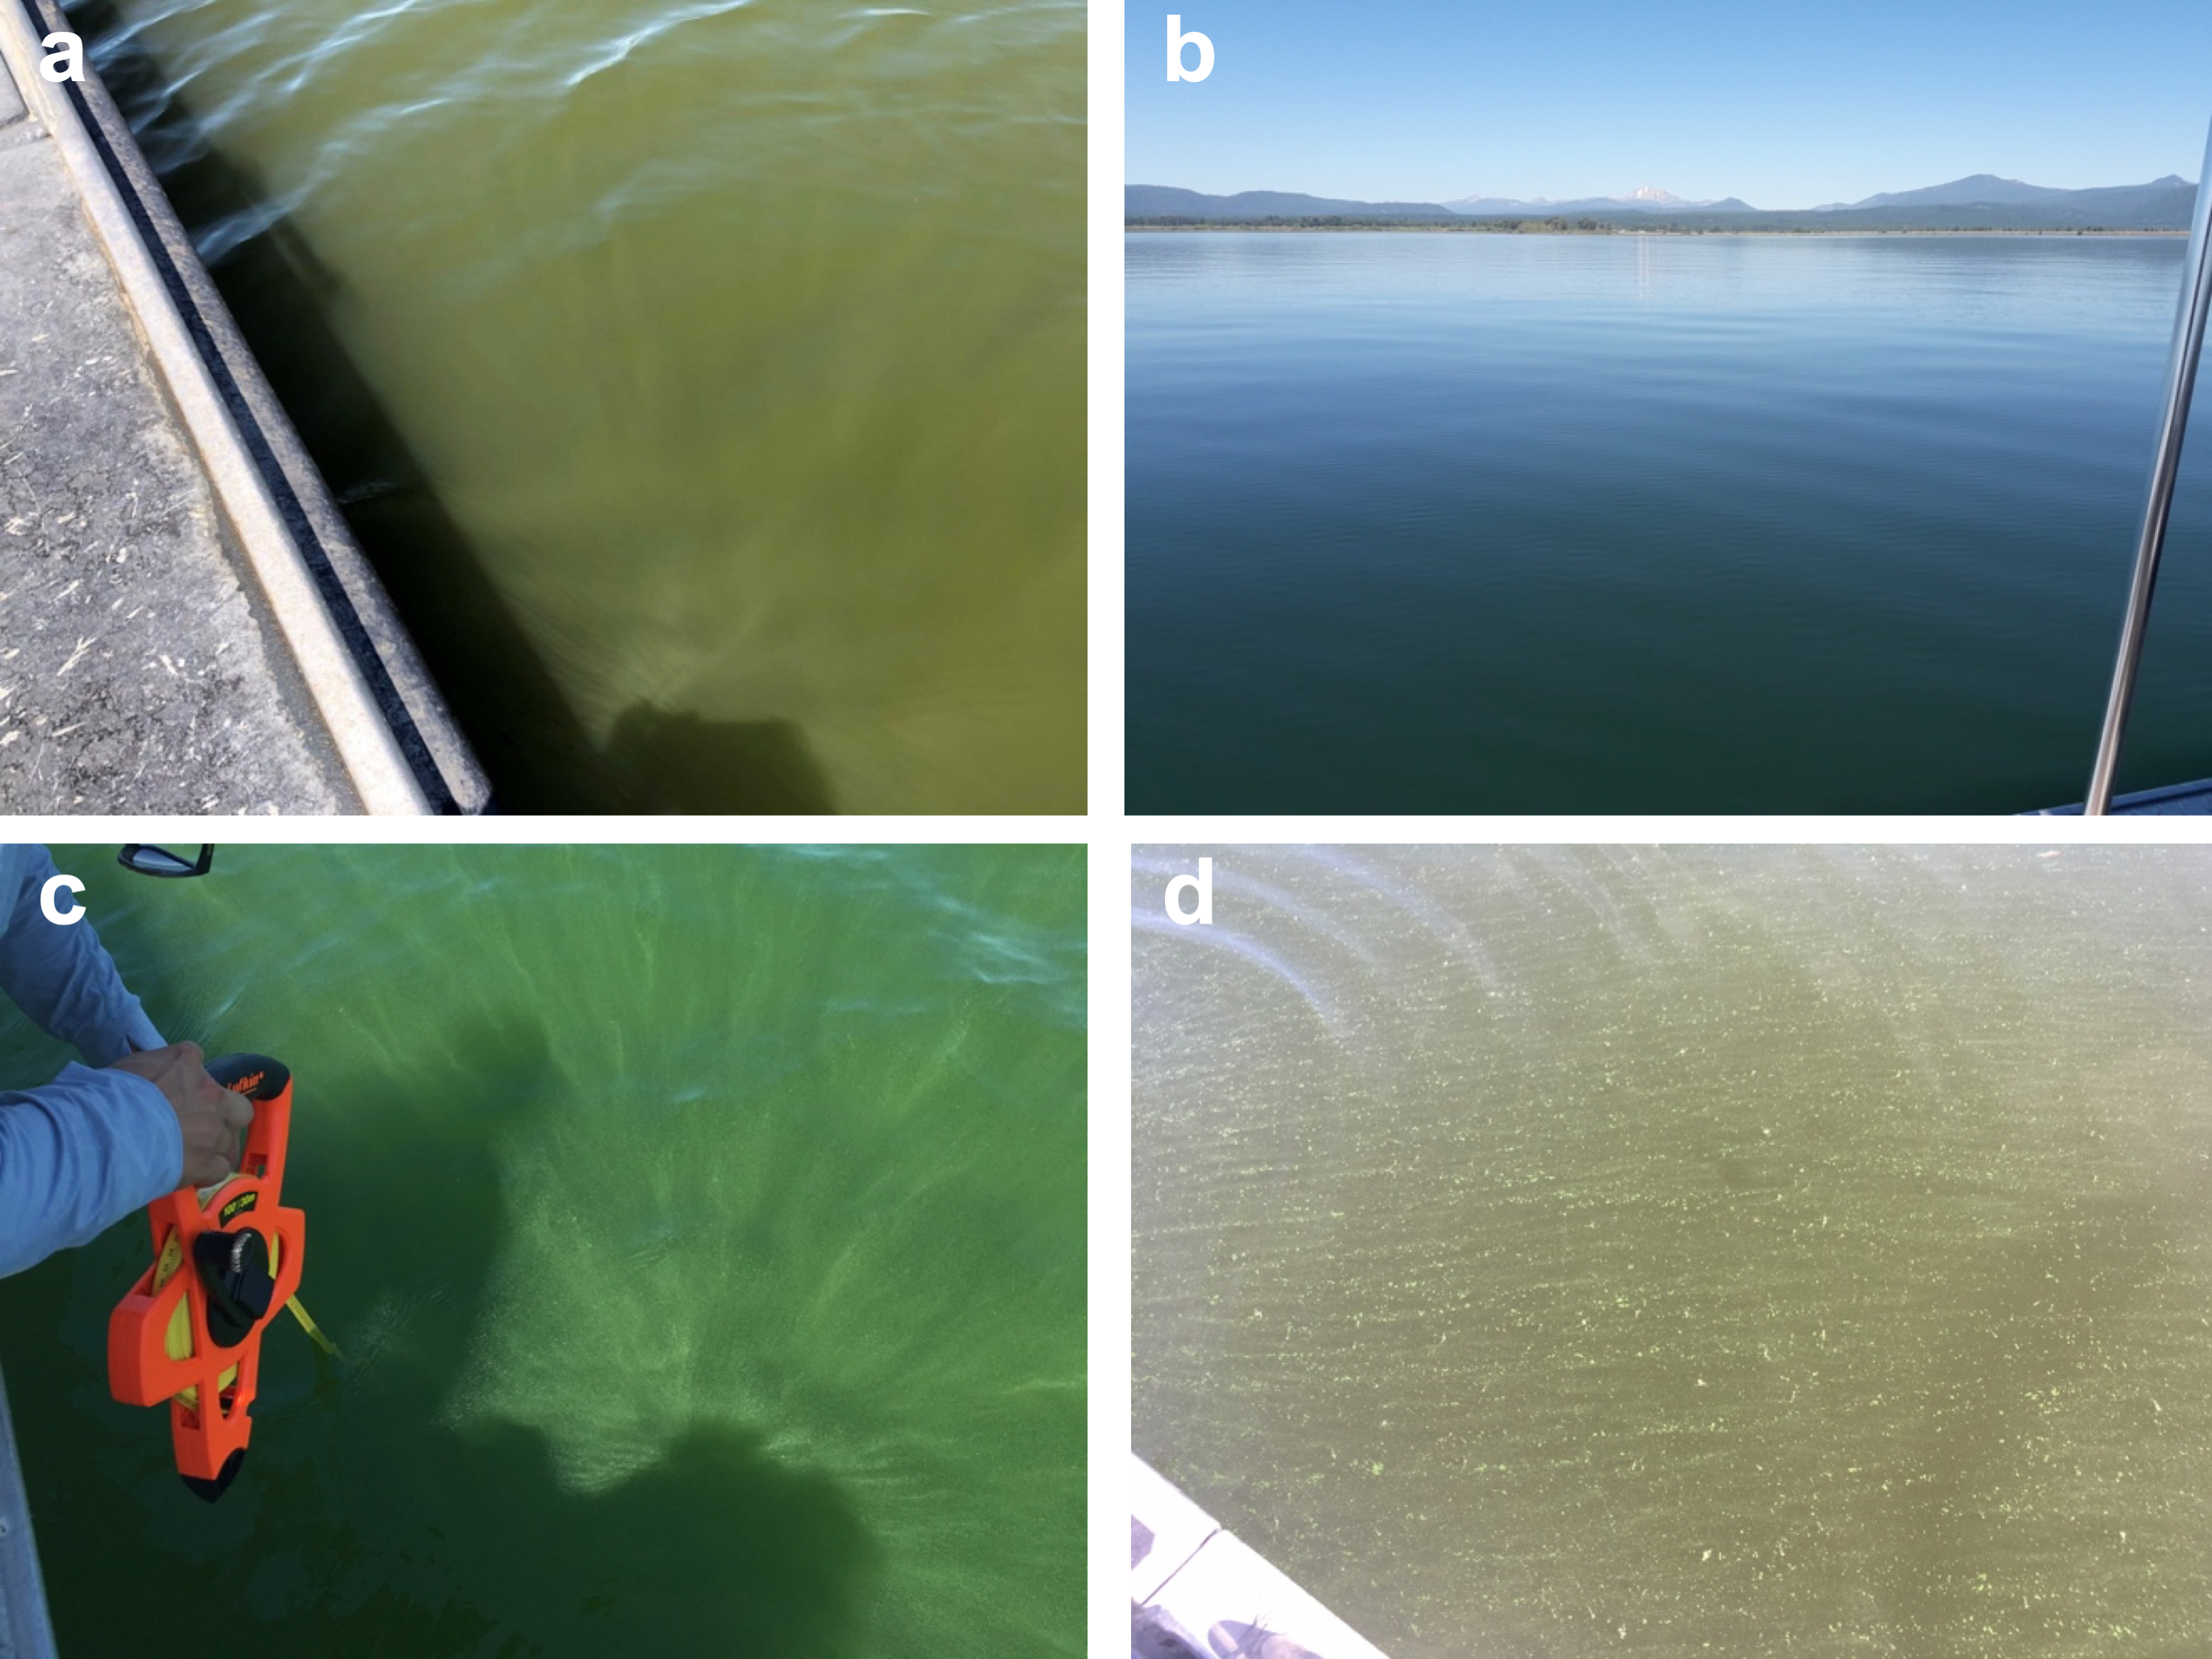
\includegraphics[width=41.64in]{../Data/Figures_output/Field_Photos_Figure} \end{figure}

\textbf{Figure 4.} Photographs of water conditions on sampling days.
\textbf{a}) Lake San Antonio, \textbf{b}) Lake Almanor, \textbf{c})
Clear Lake Aug-16, and \textbf{d}) Clear Lake Oct-08.

\paragraph{\texorpdfstring{\emph{Remote sensed reflectance
spectra}}{Remote sensed reflectance spectra}}\label{remote-sensed-reflectance-spectra}

The field collected remote sensed reflectance (R\textsubscript{rs}) data
showed chlorophyll-a absorbption decrease \textasciitilde{}681 nm in
samples with high chlorophyll-a concentrations, Clear Lake and Lake San
Antonio (Fig. 5 top row). Lake Alanor had the lowest chl-a concentratios
(Fig. 2) and little chlorophyll a absorption an no phycocyanin
absorption. San Pablo Reservoir demonstrated lower chlorophyll
absorption. The Lake Almanor and San Pablo Reservoir
CI\textsubscript{mod} values were below satellite detection levels due
to an absence of the phycocyanin absorption at 620 nm.

\begin{figure}
\includegraphics[width=0.5\linewidth]{../Data/Figures_output/RRS_Spectra_Figure} \end{figure}

\textbf{Figure 5.} Field collected remote sensed reflectance
(R\textsubscript{rs}) spectra. Waterbody name, date, and pixel are given
for each spectra. Vertical dashed lines mark OLCI band center
wavelengths at 620, 665, 681, and 709 nanometers (nm).

\paragraph{\texorpdfstring{\emph{SS(665)
values}}{SS(665) values}}\label{ss665-values}

All 142 field SS(665) values were \textless{}0 suggesting that
cyanobacteria were not present at any of the field sampling locations
(Fig. 6). The range of SS(665) values was -0.0025 to -0.000071.

\begin{figure}
\includegraphics[width=27.08in]{../Data/Figures_output/ss665_hist} \end{figure}

\textbf{Figure 6.} Histogram of all SS(665) values (N = 142).

\paragraph{\texorpdfstring{\emph{CI
values}}{CI values}}\label{ci-values}

CI values will be shown in the results, since CI\textsubscript{cyano}
values would all be zero, because CI\textsubscript{cyano} values were
all \textless{}0. Variance among the triplicate measurements within a
site was low (Fig. 7). Lake Almanor and San Pablo reservoir had CI
values \textless{}0 suggesting no cyanobacteria present in the
waterbody. All other waterbodies had positive CI values, possibly
suggesting the presence of cyanobacteria, though other water quality
conditions can generate positive CI values in the absence of
cyanobacteria.

\begin{figure}

{\centering \includegraphics[width=27.08in]{../Data/Figures_output/ci_wbd} 

}

\end{figure}

\textbf{Figure 7.} Field collected CI values from all sampling
locations.

The field data estimated higher cyanobacterial abundances than the
satellite data (Fig. 8). Both the satellite and field data estimated no
cyanobacteria at Lake Almanor and San Pablo Reservoir. The field and
satellite data were also well correlated in estimating cyanobacterial
abundances at Clear Lake on Aug-07 and a single pixel on 16-Aug.
However, all field R\textsubscript{rs} spectra and visual observations
from Lake San Antonio, Clear Lake 08-Oct, and two pixels at Clear Lake
16-Aug suggested cyanobacterial abundances, while the satellite
estimated no cyanobacteria. If the field derived CI\textsubscript{cyano}
were used, instead of CI, then all field data would have
CI\textsubscript{cyano}=0. This would more closely match the satellite
data, since the majority of the satellite pixels were non-detects. The
field CI values related correlated better with chlorophyll-a levels
(Fig. 9), than with the the satellite CI values.

\begin{figure}
\includegraphics[width=0.5\linewidth]{../Data/Figures_output/ci_fs} \end{figure}\begin{figure}
\includegraphics[width=0.5\linewidth]{../Data/Figures_output/ci_mod_fs} \end{figure}

\textbf{Figure 8.} Comparison of field and satellite data. Top panel)
Field CI\textsubscript{cyano} values and Satellite
CI\textsubscript{cyano} values. Bottom panel) Field
CI\textsubscript{mod} values and satellite CI\textsubscript{mod} values
(modified scale 1-1000. Colors show the waterbody and sampling date. The
1:1 line is dashed.

\begin{figure}

{\centering \includegraphics[width=0.6\linewidth]{../Data/Figures_output/ci_mod_chla} 

}

\end{figure}

\textbf{Figure 9.} Comparison of field CI\textsubscript{mod} and
chlorophyll-a. Colors show the waterbody and sampling date.

There was no strong relationship between SS(665) and
CI\textsubscript{mod} (Fig. 10). Surprisingly, Lake Almanor, which had
the lowest chl-a concentrations had SS(665) values comparable to Clear
Lake, which had visible cyanobacterial colonies.

\begin{figure}

{\centering \includegraphics[width=0.6\linewidth]{../Data/Figures_output/ss665_CImod} 

}

\end{figure}

\textbf{Figure 10.} Relationship between SS(665) and field
CI\textsubscript{mod} for all waterbodies.

\subsection{\texorpdfstring{\textbf{Discussion}}{Discussion}}\label{discussion}

\begin{itemize}
\item
  Are the CI value equations and interpretations correct?
\item
  Are the SS(665) values \textless{}0 expected or reasonable? Is this
  surprising?
\item
  The CI\textsubscript{mod} values from the field were all
  \textless{}60, which on a scale of 1-1000 are relatively low. Do these
  results suggest that there is a lot of noise in the satellite data at
  low CI-od values, where the satellite is more prone to generate false
  negative pixels when CI\textsubscript{mod} \textless{}60.
\item
  SFEI obtains CI\textsubscript{cyano} from NOAA. It would be nice to
  see the corresponding CI and CI\textsubscript{cyano} values for each
  waterbody to make more comparisons between the field and satellite
  data. Though SFEI also gets CI and CInoncyano, they exclude it from
  their data processing workflow, and so there is more data processing
  work required to obtain these values.
\end{itemize}

\subsection{References}\label{references}

Lunetta, R, et al. 2015. Evaluation of cyanobacteria cell count
detection derived from MERIS imagery across the eastern USA.
\emph{Remote Sensing of the Environment} 157:24-34

Matthews, M, et al. 2012. An algorithm for detecting trophic status
(chlorophyll-a), cyanobacterial-dominance, surface scums and floating
vegetation in inland and coastal waters. \emph{Remote Sensing of
Environment} 124:637-652

Mobley, C. 1999. Estimation of the remote-sensing reflectance from
above-surface measurements. \emph{Applied Optics} 38(36):7442-7455.

Tomlinson, S, et al. 2016. Relating chlorophyll from
cyanobacteria-dominated inland waters to a MERIS bloom index.
\emph{Remote Sensing Letters} 7(2):141-149

Wynne, T, et al. 2008. Relating spectral shape to cyanobacterial blooms
in the Laurentian Great Lakes. \emph{International Journal of Remote
Sensing} 29(12):3665-3672

Wynne, T, et al. 2018. Harmful Algal Bloom Forecasting Branch Ocean
Color Satellite Imagery Processing Guidelines. \emph{NOAA Technical
Memorandum} NOS NCCOS 252. \url{doi:10.25923/twc0-f025}

\end{document}
